\section{Ejercicio 2}
\subsection{Introducción}
\noindent \underline{\textbf{Contexto}}

Estamos frente a un nuevo juego de mesa, que es una alternativa al ajedrez tradicional. Se usa un tablero de ajedrez especial, que puede tomar dimensiones de \textit{n $\times$ n} casillas, y solo se juega con caballos blancos. El unico movimiento permitido es desplazar dichos caballos, de la forma tradicional del de ajedrez (o sea en L), y con una regla adicional que permite que varios caballos puedan compartir la misma ubicacion.

Los caballos se colocan al inicio del juego en determinadas posiciones, las cuales son arbitrarias, y se pueden llegar a dar casos donde hay mas de un caballo inicialmente en la misma ubicacion. El objetivo del juego es ir moviendo los caballos, y lograr ubicar todos los caballos en un solo lugar usando la menor cantidad de movimientos posibles.

\noindent \underline{\textbf{El problema a resolver}}

Debemos diseñar un algoritmo, que dado el tamaño del tablero \textit{n}, la cantidad de caballos \textit{k} y las posiciones \textit{f} \textit{c} (fila y columna respectivamente) iniciales de estos dentro del tablero, calcule el mejor casillero para elegir ubicar a dichos caballos, de tal manera que minimice la cantidad de movimientos realizados. 

El algoritmo debe devolver el casillero elegido y la cantidad de saltos realizados en total, en caso de no tener solucion, simplemente devolver la palabra \textbf{no}. Este algoritmo debera tener una complejidad temporal de a lo sumo \textit{$O(k \times n^2)$}.

\noindent \underline{\textbf{Ejemplos}}
\begin{multicols}{2}
\begin{enumerate}[leftmargin=0.5cm]
\item n = 3, k = 3

Fila1 = 1 Columna1 = 2\\
Fila2 = 3 Columna2 = 1\\
Fila3 = 3 Columna3 = 3

Resultado: 1 2 2

\item n = 3, k = 3

Fila1 = 1 Columna1 = 1\\
Fila2 = 2 Columna2 = 3\\
Fila3 = 2 Columna3 = 2

Resultado: no

\item n = 5, k = 4

Fila1 = 1 Columna1 = 1\\
Fila2 = 4 Columna2 = 2\\
Fila3 = 1 Columna3 = 5\\
Fila4 = 4 Columna4 = 4

Resultado: 2 3 4

\item n = 8, k = 8

Fila1 = 1 Columna1 = 1\\
Fila2 = 7 Columna2 = 4\\
Fila3 = 3 Columna3 = 7\\
Fila4 = 5 Columna4 = 3\\
Fila5 = 3 Columna5 = 8\\
FIla6 = 4 Columna6 = 5\\
Fila7 = 8 Columna7 = 1\\
Fila8 = 7 Columna8 = 7

Resultado: 5 3 14
\end{enumerate}

\columnbreak

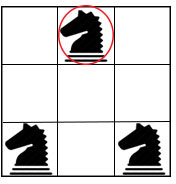
\includegraphics[scale=0.20]{img/knight3x3_1.jpg}\\\\\\

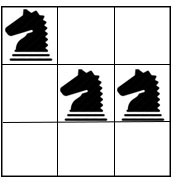
\includegraphics[scale=0.20]{img/knight3x3_2.jpg}\\\\\\

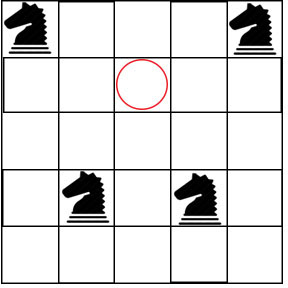
\includegraphics[scale=0.20]{img/knight5x5.jpg}\\\\

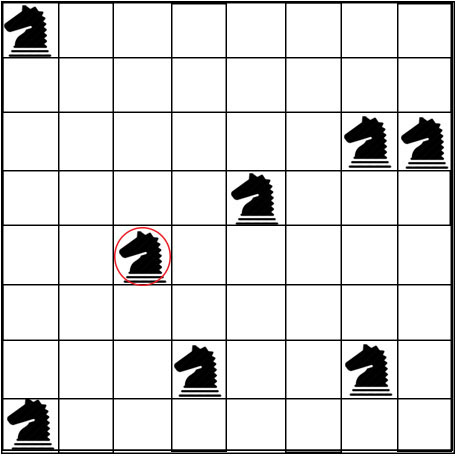
\includegraphics[scale=0.20]{img/knight8x8.jpg}
\end{multicols}

\newpage
\subsection{Desarrollo}

Para resolver el problema presentado, se analizaron diferentes propiedades:

Se puede interpretar al tablero como un grafo, con sus nodos las coordenadas, y sus ejes los desplazamientos que puede realizar un caballo. Dado que sabe que las opciones de desplazamiento de un caballo es como maximo 8, entonces la cantidad de ejes por nodo va a ser a lo sumo 8.

\begin{center}
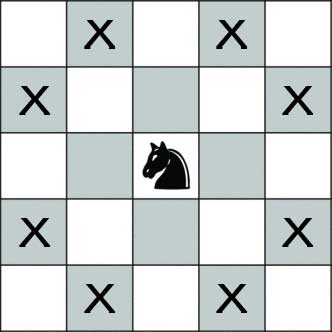
\includegraphics[scale=0.25]{img/knight.jpg}
\end{center}

Se puede ver ademas que para el problema se pide una complejidad no superior a \textit{O(k · $n^2$)}, siendo k la cantidad de caballos y $n^2$ el tamaño del tablero, lo cual da una sospecha que para cada caballo se tengan que realizar operaciones con complejidad \textit{O($n^2$)}.

\bigskip
Algunas definiciones globales a partir de ahora:
\begin{enumerate}
\item \textbf{Tablero}, \textbf{Matriz} y \textbf{Grafo} se van a referir a lo mismo, al tablero asociado al problema.
\item \textbf{Caballo}, \textbf{Coordenada}, \textbf{Posicion}, \textbf{Nodo}, y todos sus sinonimos en grafos van a significar lo mismo.
\item \textbf{Salto}, \textbf{Desplazamiento}, \textbf{Eje}, y todos sus sinonimos en grafos van a significar lo mismo.
\item \textbf{Distancia} a la longitud del camino mas corto de una posicion a otra, es decir, su definicion en grafos.
\end{enumerate}

\bigskip
Se propone entonces, una funcion que calcule la matriz de distancias para cada caballo, la cual en cada posicion del tablero, va a tener su distancia del caballo.

\bigskip

\noindent \underline{\textbf{Matriz de Distancias}}

Esta función sirve para calcular el camino mínimo entre una posición del tablero inicial, y todas las que estan alrededor, sin embargo tiene funcionalidad limitada ya que en términos de este ejercicio, solo hace falta la distancia mínima y no el camino mínimo.

Se recibe una matriz con \textit{n $\times$  n} casilleros inicializados con la distancia -1, para indicar que aun no se los revisaron. Le asignamos a la matriz en la posición del caballo la distancia 0, debido a que es de la cual se arranca, y se agrega dicha posición a una cola, en la cual se van a guardar todos los nodos pendientes para procesar. 

Por cada nodo perteneciente a esta cola, va a desencolarlo y análizar todos sus nodos adyacentes:
\begin{itemize}
\item[•]Si aun no fueron analizados, se les escribe la distancia del nodo actual mas uno, debido a que requiere un salto mas para llegar hasta ahi, y se lo guarda en la cola.
\item[•]Si ya fueron analizados, se revisa si la nueva distancia es menor que la que ya tenía, en caso positivo se la actualiza.
\end{itemize}

Como este análisis involucraría todas las posiciones, en principio va a tener una complejidad de $\Omega(n^2)$, en la sección de complejidad se verá que esto de hecho es $\Theta(n^2)$. 
\bigskip

\begin{center}
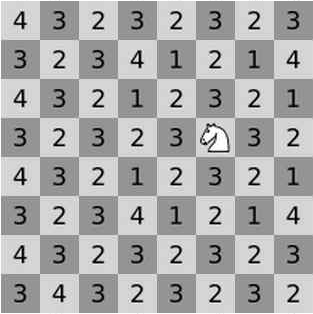
\includegraphics[scale=0.5]{img/knight_movements.png}
\end{center}
\newpage
\begin{lstlisting}
void MatrizDistancias(Tablero& tablero, Coordenada caballo)

	tablero[caballo.x][caballo.y] = 0
	Cola<Coordenada> cola
	cola.encolar(caballo)
	
	Mientras cola tenga elementos
	
		Coordenada v = cola.desencolar()
		
		Para toda coordenada u adyacente a v
			Si tablero[u.x][u.y] == -1
				tablero[u.x][u.y] = tablero[v.x][v.y] +1
				cola.enconlar(u)	
			Fin si
		Fin Para
		
	Fin Mientras
Fin
\end{lstlisting}

\noindent \underline{\textbf{Resolución General}}

Se genera para cada caballo una matriz de \textit{n $\times$  n} casillas, inicializado todas sus posiciones en -1 para indicar que aun no se revisaron, y se pasa dicha matriz a una funcion que calcula la matriz de distancias asociada al caballo.

Se suman todas estas matrices en una sola, y se busca el minimo valor dentro de ella. Este minimo valor va a ser la suma de todas los saltos requeridos combinados de los caballos para llegar hasta el, que es lo que el algoritmo debe resolver. 

Una manera de mejorar la complejidad espacial es mantener una matriz cache para ir guardando la suma acumulada de las sumas hasta ese momento.

Para el caso donde es con tableros con n $<$= 3, debido a que no se puede llegar a todos los casilleros dada una posicion de un caballo, se los revisa independientemente. Como estos casos son limitados, no aportan a la complejidad.
\bigskip

\begin{lstlisting}
Tablero cache <- Crear matriz de tamano n x n con valor 0

Para todo c en caballos
	Tablero distancias <- Crear matriz de tamano n x n con valor -1
	MatrizDistancias(distancias, c)
	cache += distancias
Fin Para
	
Buscar en el tablero cache la coordenada con el minimo valor
\end{lstlisting}

\bigskip
El pseudocódigo puede diferir levemente del código actual, pero se lo hizo asi para que sea mas entendible y se omitieron algunos detalles innecesarios, para consultarlos, ver el código.

\newpage

\subsection{Correctitud}
En este apartado veremos que la solución presentada para resolver el ejercicio, es correcta. Empecemos por analizar la correctitud de la funcion que calcula la matriz de distancias, dado un punto de origen, tiene que calcular la longitud minima(distancia) de salto para cada posicion en el tablero.

\bigskip
\noindent \underline{\textbf{Matriz de Distancias}}

En esta parte se usa el algoritmo de BFS (Breadth-First Search), adaptado para que vaya escribiendo la distancia a cada nodo a medida que va recorriendolos. Esto usa fuertemente que el peso de todas las saltos es de 1, la idea intuitiva es que debido a que recorre a lo ancho el grafo asociado al tablero, y que el peso de las aristas es siempre 1, por cada iteración va recorriendo en forma circular el grafo, ampliando el radio cada vez que los el valor de los nodos en la cola cambia, hasta abarcar a todos los nodos (que no hayan mas nodos sin marcar). Entonces como el peso de los saltos es de uno, el anterior obligatoriamente tiene que estar en el circulo del radio actual -1.

Se puede ver facilmente en el algoritmo que la cola que se usa va a estar siempre ordenada de menor a mayor, ya que primero se va a encolar los nodos adyacentes al origen (valor 1), luego a los adyacentes sin analizar de los anteriores (valor 2), y asi sucesivamente. Llamaremos a partir de ahora entonces iteración a cada vez que se acaba determinado valor en la cola, o sea que aumenta el radio de busqueda.

\textbf{Ejemplo del recorrido del algoritmo:}

\begin{enumerate}
\item Escribe 0 en la posicion origen
\item 1era iteración: Escribe en todos los adyacentes al origen el valor 1, ya que ninguno fue recorrido aun
\item 2da iteración: Escribe en todos los adyacentes a los nodos de valor 1 que aun no fueron analizados el valor del nodo actual +1 (o sea 2)
\item 3ra iteración: Escribe en todos los adyacentes a los nodos de valor 2 que aun no fueron analizados el valor del nodo actual +1 (o sea 3)
\item k-esíma iteración: Escribe en todos los adyacentes a los nodos de valor k-1 que aun no fueron analizados el valor del nodo +1 (o sea k)
\end{enumerate}

Se puede ver entonces que en cada paso, efectivamente se esta poniendo la distancia mínima en todos los nodos al nodo origen. Pero esto aun no esta formalizado.

\bigskip
\textbf{Lema/Invariante:}

Para la k-esíma iteración, para obtener la longitud minima de los nodos k al punto de origen, el predecesor directo de estos es algun nodo de la iteración k-1.

Demostremos esto por el absurdo, dado un nodo \textbf{v} en la k-esíma iteración, existe \textbf{u} nodo predecesor con distancia menor a los nodos pertenecientes a \textbf{K-1}, siendo \textbf{K-1} el conjunto de nodos analizados de la k-1esíma iteración. Esto implicaría que \textbf{u} pertenezca a \textbf{Q}, siendo \textbf{Q} el conjunto de nodos aún no analizados.

Según nuestro algoritmo: 
\begin{itemize}
\item[•]La unica manera de alcanzar \textbf{u} es en alguna iteracion $>=$ k, ya que sino este pertenecería al conjunto \textbf{K-1}.
\item[•]El valor de esta iteración va a ser k + c , para algún c $>=$ 0.
\item[•]En cada iteración, los nodos que se analizan quedan con el valor del numero de iteración.
\item[•]Por los dos puntos anteriores, valor de los nodos de la iteración k + c va a ser k + c. 
\end{itemize}

\bigskip
Entonces queda:

\begin{center}
 $d(u) < k \Longleftrightarrow k + c < k$ ¡Absurdo!
\end{center}

\bigskip
El absurdo provino de suponer que existe algún nodo con valor menor a k en los nodos aún no analizados, por lo tanto el predecesor obligatoriamente tiene que pertenecer a los nodos ya analizados de la K-1esíma iteración. Estos nodos siempre existen ya que desde la iteración 1 existe el nodo origen con distancia 0.

Entonces si se hace esto desde 0 hasta k, queda que todos los nodos de valor $<=$ k tienen la longitud mínima al punto de origen, quedando demostrado el lema.

\newpage
\textbf{Teorema/Invariante y terminación:}

Todos los nodos tienen la mínima longitud al punto de origen. Esto seria el invariante cuando alcanza la última iteración básicamente, cuando ya no hay mas nodos sin analizar.

Con esto queda demostrada la correctitud de la funcion que calcula la matriz de distancias.

\bigskip
\noindent \underline{\textbf{Correctitud General}}

Gracias a lo probado anteriormente, se ve facilmente que sumar todas las matrices de distancia correspondientes a cada caballo, nos va a dar una suma de matrices en la cual va a estar la cantidad de saltos mínima necesaria a realizar para llegar a cada casillero. Entonces lo que se hace es buscar el mínimo en esta matriz, y devolver su posicion y valor.

Siguen existiendo casos particulares en los que puede que no haya solución aplicando esta estrategia, estos son los que tienen tamaño de matriz con n $<=$ 3, a partir de n $>$ 3 con cualquier caballo se puede llegar a cualquier posición.

\begin{enumerate}
\item[•] n == 3, se revisa que si tiene caballos en el medio, que esten todos ahí, sino no tiene solución.
\item[•] n == 2, se revisa que si tiene caballos en alguna posición, que esten todos ahí, sino no tiene solución.
\item[•] n == 1, caso trivial, siempre tiene solucion y es única.
\end{enumerate}

Entonces quedan abarcados y demostrados todos los casos que se pueden presentar, quedando demostrada la correctitud del algoritmo.

\subsection{Complejidad}
Para analizar la complejidad del algoritmo, se va a analizar primero la funcion Matriz de Distancias, para luego poder ver la complejidad del algoritmo completo.

\bigskip
\noindent \underline{\textbf{Matriz de Distancias}}

Se recibe una matriz con $n^2$ posiciones, todas con el valor -1. Se le asigna 0 a la posicion original y se lo agrega a una cola. Luego se analiza cada posicion en la cola: se revisa todas las adyacencias a dicha posicion, que en el peor caso son 8, ya que un caballo como maximo tiene 8 posibles posiciones para saltar, quedando que este analisis cuesta \textbf{\textit{$\Theta$(1)}}.

Dicho analisis lo hace una y solo una vez para cada posicion en el tablero ($n^2$), esto es debido a que las posiciones ya revisadas no se vuelven a repetir: va eligiendo las posiciones que estan marcadas con -1 para encolarlas y desmarcarlas, luego no vuelven a valer mas -1. La cola que se usa es una cola lineal, por lo tanto tiene complejidad constante para el encolado y desencolado.

Entonces este algoritmo analiza $n^2$ posiciones, y como dicho analisis cuesta \textbf{\textit{$\Theta$(1)}}, la complejidad temporal de la funcion que calcula la matriz de distancias queda \textbf{\textit{$\Theta$($n^2$)}}

\bigskip
\noindent \underline{\textbf{Complejidad General}}

Realicemos un analisis de cada paso:
\begin{itemize}
\item[•]Crear un tablero cache de $n^2$ posiciones con el valor 0: \textbf{\textit{$\Theta$($n^2$)}}
\item[•]Para cada caballo, se crea un tablero de $n^2$ posiciones con el valor -1, se calcula su matriz de distancias asociada, y luego se la suma al tablero cache: \textbf{\textit{$\Theta$($k \times n^2$)}}
\item[•]Buscar al minimo en el tablero cache con todas las sumas: \textbf{\textit{$\Theta$($n^2$)}}
\end{itemize}

Sumando todas las complejidades, queda entonces que este algoritmo tiene una complejidad temporal final de \textbf{\textit{$\Theta$($k \times n^2$)}}

Para el caso en el que el tamaño del tablero sea menor o igual a 3 $\times$ 3, queda absorbido por la complejidad general ya que lo resuelve en complejidad temporal lineal respecto de k.
\newpage
\subsection{Experimentación}
Para el proceso de experimentación del problema se plantearon distintos escenarios de test para corroborar que el algoritmo propuesto funcionara correctamente y que la cota de complejidad encontrada y justificada en la sección anterior, en la práctica, se cumpliera.

En cuanto a qué casos testear, nuestro algoritmo no presenta casos “border”. Es decir, no tiene un peor/mejor caso, sino que para cualquier instancia cargada, realizará el mismo procedimiento, ya que las posiciones de los caballos no afecta el tiempo de computo del algoritmo, tomando \textbf{$\Theta$\textit{(k $\times$ $n^2$)}}.

En cada prueba se tomaron métricas para la posterior evaluación del algoritmo en la práctica. Notar que la medición no contempla tiempos de entrada/salida de datos, sino que contempla solamente el núcleo del algoritmo.

Se diseñó un programa que dado un numero i de instancias, n de edificios y k de caballos, genera i instancias aleatorias con tableros de tamaño n x n, y k caballos aleatorios para probar el algoritmo.

Para cada instancia experimentada, se la hizo ejecutar 100 veces y se tomo el valor mínimo, esto es debido a que dado que el CPU de la computadora utilizada para tomar los tiempos no está atendiendo únicamente a nuestro proceso, realizar una sola vez cada prueba podría darnos valores que no son cercanos a los reales, entonces para minimizar el márgen de error, se realiza este procedimiento. Notar que tomar el mejor mínimo no es una mala decisión, ya que mientras más chico sea, más cerca estamos del valor real de tiempo que toma el algoritmo para una instancia dada.

Explicado esto, para cada tamaño de entrada se realizaron 100 pruebas con instancias aleatorias distintas, las cuales devuelven el mejor valor, de las cuales se calcula el promedio de estos 100 valores. 

Se realizaron experimentos primero fijando el tamaño del k y variando el n, y viceversa, para poder detectar la dependencia temporal del algoritmo sobre cada variable

En todos los casos se pudo comprobar que la práctica refleja lo expuesto en incisos anteriores. A continuación presentamos los gráficos 2D que reflejan las pruebas realizadas. 

\bigskip
\noindent 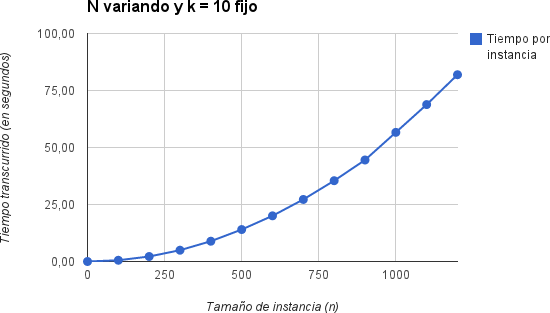
\includegraphics[scale=0.45]{img/grafico_n.png}
\noindent 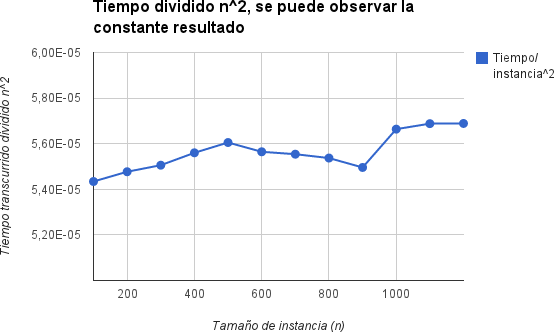
\includegraphics[scale=0.45]{img/grafico_n2.png}

\bigskip
\noindent 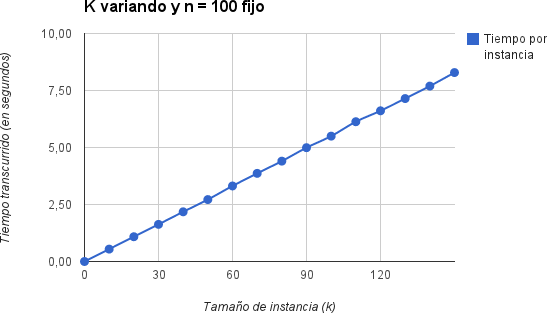
\includegraphics[scale=0.45]{img/grafico_k.png}
\noindent 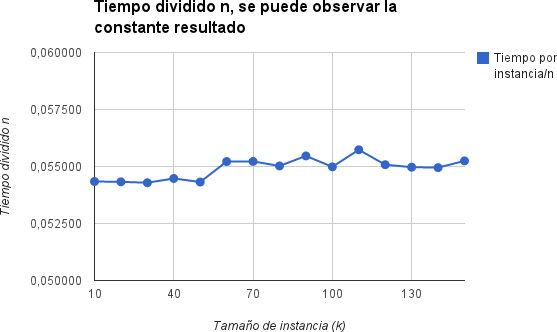
\includegraphics[scale=0.45]{img/grafico_k2.png}

\bigskip
Los gráficos de la izquierda son las mediciones que se hicieron, y los de la derecha son los de la izquierda divididos por $n^2$ y k, respectivamente, formando una oscilacion de una recta. Se puede entonces ver, que los experimentos reflejan lo demostrado en la teoria.